\section{Cross talk measurements}

To demonstrate the crosstalk between adjacent pixels on the MAPMTs, we collected data where the whole PMT face was masked with a sheet of black paper, and a single 3mm diameter hole was punctured over the center of one pixel. Despite the majority of the laser light being incident on the single unmasked pixel, we observed signals above pedestal in the surrounding pixels as well. Fig.~\ref{fig:H12700pinhole} shows the measured spectra for the central and neighboring pixels when the puncture hole was directly above pixel 29. There are two types of events we see in this data set for the pixels surrounding the illuminated pixel. The first is the electronic crosstalk resulting from the electron cascade in the central pixel. The signal measured in a neighboring pixel is directly proportional to that which is measured in the central pixel. In Fig.~\ref{fig:H12700pinhole}, these types of events are characterized by a shoulder attached to the right of the pedestal. This is most prominently seen in the spectrum for the pixel directly to the right of the central pixel of Fig.~\ref{fig:H12700pinhole} (pixel 30). Because of the strong correlation of the crosstalk to the central pixel, these types of events can be identified and removed from the data offline. More will be discussed on this later.

The second type of event observed in the neighboring pixels of this data comes from the displacement of the photoelectron emitted by the photocathode. When the incident photon hits pixel 29, there is some probability that the emitted photoelectron is detected by one of the neighboring pixels. Because there is no correlation with the central pixel for these events, there is no way to identify these signals on an event-by-event basis. In Fig.~\ref{fig:H12700pinhole}, the spectra drawn in red have the additional cut applied that the signal in the central pixel should be greater than 10$\sigma$ above the pedestal. With this cut applied, the number of events beyond the crosstalk shoulder in the neighboring pixels is reduced by more than an order of magnitude.

\begin{figure}
	\centering
	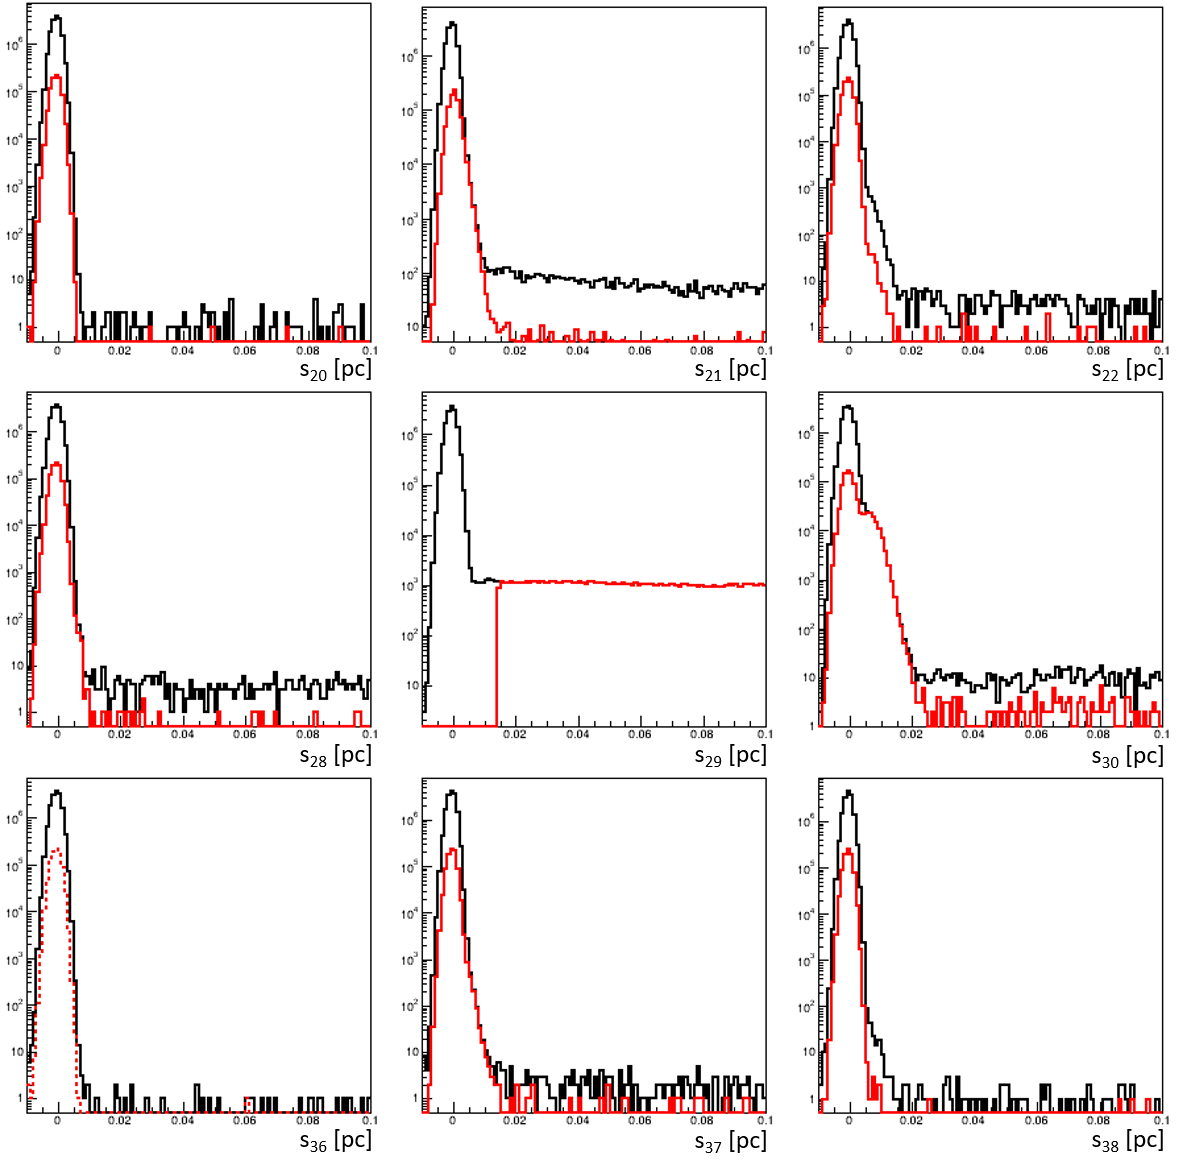
\includegraphics[width=\linewidth]{figures/H12700_3mm_mask_config5_ct.png}
	\caption{Black: the charge spectra for pixel 29 of a typical H12700 MAPMT and the surrounding pixels when only pixel 29 was illuminated by the laser light. Red: the same spectra with the cut that the signal in pixel 29 is 10$\sigma$ above pedestal.}
	\label{fig:H12700pinhole}
\end{figure}

Using this masking scheme, we collected data with different pixels unmasked and measured the fraction of events where we observe cross talk in the neighboring pixels. Fig.~\ref{fig:H12700_ct_ratio} shows these fractions for four pixels. 

\begin{figure}
	\centering
	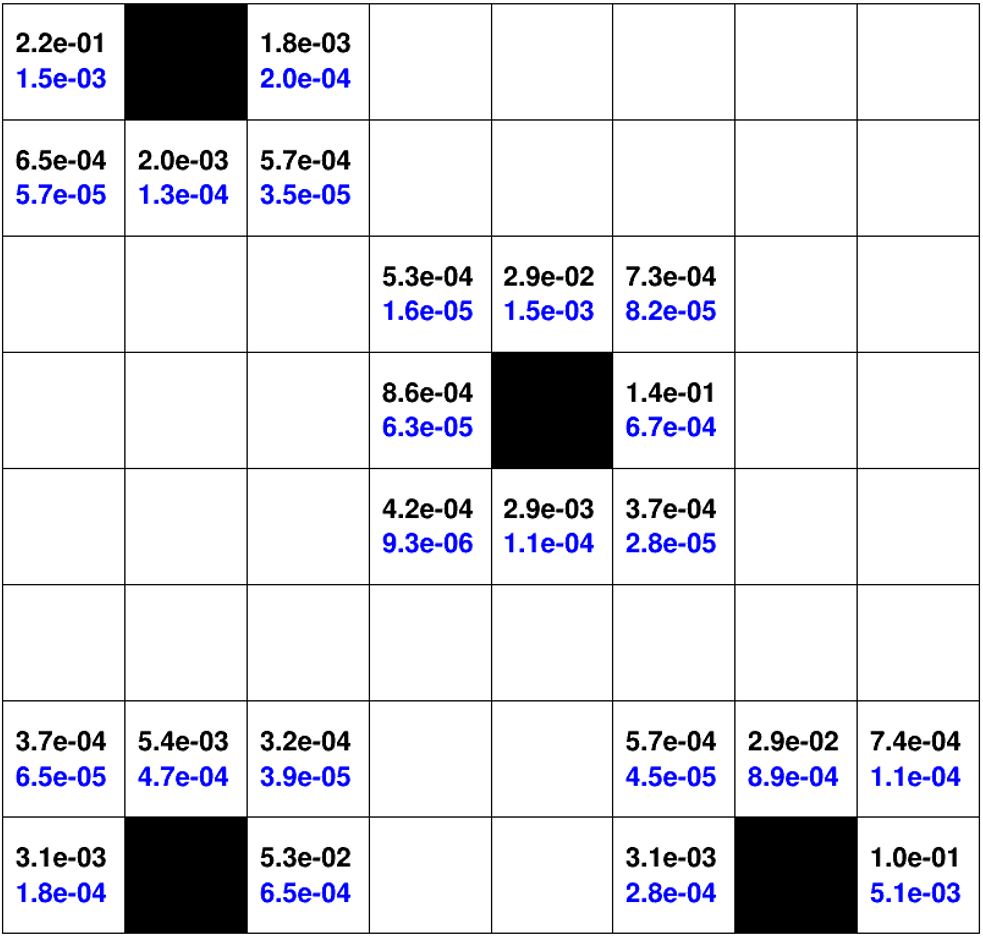
\includegraphics[width=\linewidth]{figures/H12700_ct_ratio.png}
	\caption{For each highlighted pixel a separate run was taken where only this pixel had a 3mm hole punctured in the mask covering the whole PMT face. The numbers in black in the surrounding pixels represent the fraction of events where there is crosstalk in that pixel.}
	\label{fig:H12700_ct_ratio}
\end{figure}

To properly characterize the single photoelectron spectrum for each pixel, one needs to either add a description of the crosstalk into the computational model for the s.p.e. response, or one can attempt to identify and remove these crosstalk events from the data. A simple procedure was developed and implemented to attempt the latter option. Because the amplitude of the crosstalk is linearly dependent on the amplitude of the photo-induced signal, the crosstalk events appear as linear bands in the plots showing the measured charge in one pixel as a function of the measured charge in a neighboring pixel. Fig.~\ref{fig:H12700neighbors} and Fig.~\ref{fig:H8500neighbors} show these two dimensional plots for all pixels which neighbor pixel 29 for one H12700 MAPMT and one H8500 MAPMT, respectively. The data shown in these plots were taken with the entire face of the MAPMTs illuminated by the laser light. From these two plots it is obvious that the strength of the crosstalk is vastly different between the H12700 and H8500 MAPMTs. On average, the amplitude of the crosstalk in an H12700 MAPMT is only about 2-3$\%$ of the main signal, whereas the crosstalk amplitude in an H8500 MAPMT can be as large as 50$\%$ of the main signal. As we will discuss later, this fact makes it more difficult to address the crosstalk for the H8500 MAPMTs in the mathematical description of the spe response function.

Other noteworthy features from Fig.~\ref{fig:H12700neighbors} and Fig.~\ref{fig:H8500neighbors} are that the crosstalk signals are strongest in the pixels immediately to the right and left of the pixel where light was incident. The crosstalk bands in those pixels have the largest slope. Most of the crosstalk is contained within the 4 pixels which share an edge with the illuminated pixel, as the plots for the pixels on the corners show little correlation with the charge measured in the central pixel.

\begin{figure}[hbt]
	\centering
	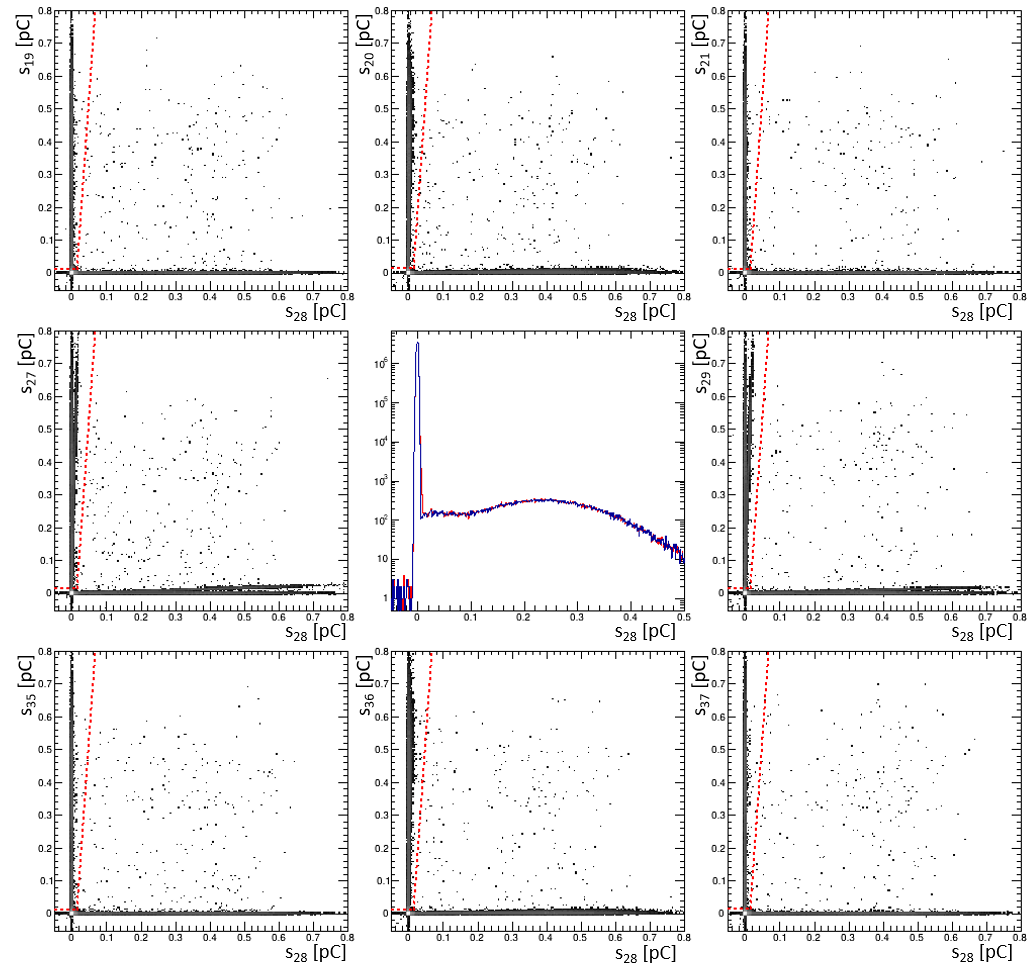
\includegraphics[width=\linewidth]{figures/H12700_ct.png}
	\caption{The charge measured in adjacent pixels is plotted as a function of the charge measured in pixel 29 for a typical H12700 MAPMT. The central plot shows the charge spectrum before (red) and after (blue) removal of the crosstalk events which are cut by the dashed (red) line on the 2-dimensional plots.}
	\label{fig:H12700neighbors}
\end{figure}
\begin{figure}[hbt]
	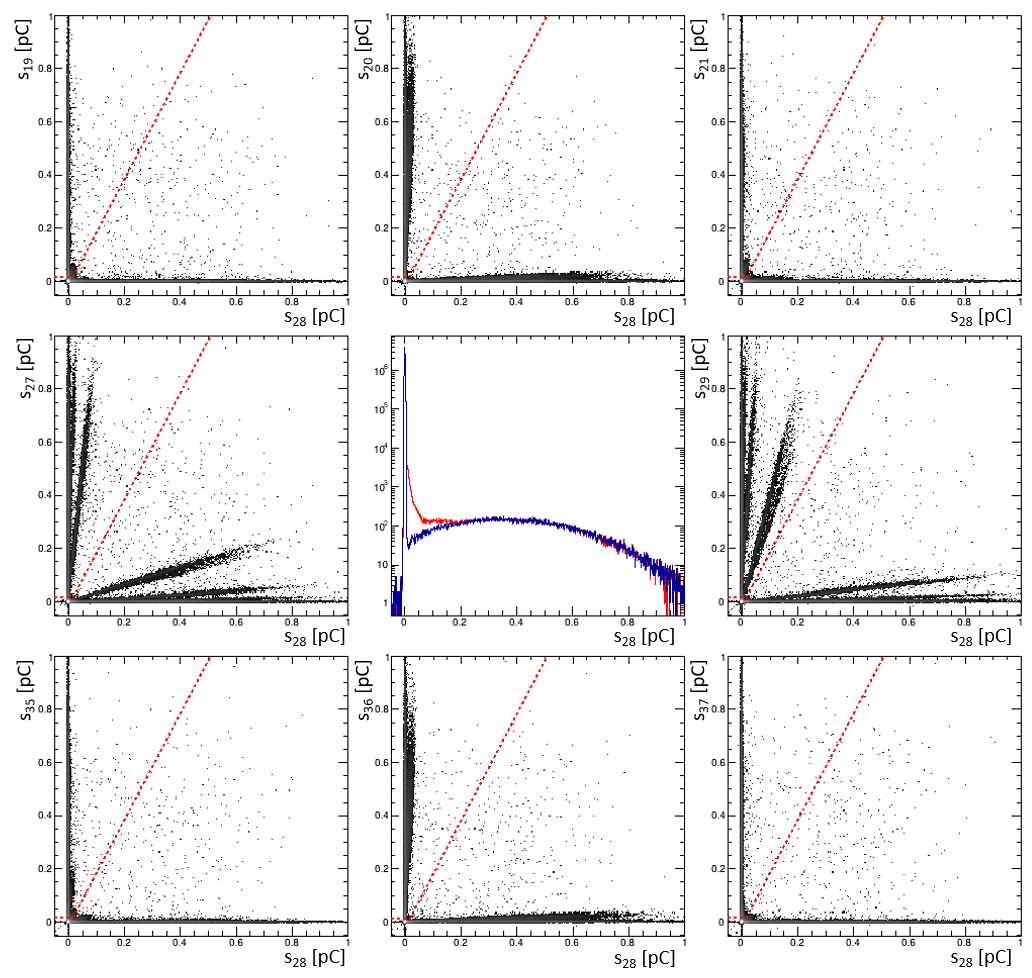
\includegraphics[width=\linewidth]{figures/H8500_ct.png}
	\caption{The charge measured in adjacent pixels is plotted as a function of the charge measured in pixel 29 for a typical H8500 MAPMT. The central plot shows the charge spectrum before (red) and after (blue) removal of the crosstalk events which are cut by the dashed (red) line on the 2-dimensional plots.}
	\label{fig:H8500neighbors}
\end{figure}

Because the crosstalk events are easily distinguished in these two dimensional plots, a cut can be placed to remove these events from the data. The cut is applied to each pixel separately, and is a linear function of the charge measured in that pixel. Specifically, the cut places a limit on the maximum charge measured in the neighboring pixels. If the maximum neighboring charge is above the cut value for the central pixel\textquotesingle s measured charge, then the event is tagged as crosstalk and is removed from the charge spectrum for the central pixel. This cut is shown as a dashed (red) line in Fig.~\ref{fig:H12700neighbors} and Fig.~\ref{fig:H8500neighbors}. The start of the cut line is placed 7$\sigma$ above the pedestal to avoid removing pedestal events. Although the slope of the crosstalk bands can vary between pixels, the slope of the cut line used here is the same for each pixel on a given PMT. 

The main drawback of this crosstalk cut is that it removes events where adjacent pixels both happen to have a photoelectron emitted from the same laser trigger. However, the fraction of these accidental coincidence events is low when the laser filter is used at the minimal setting, meaning at low light intensity this procedure can be used to provide the spe spectrum free from electronic crosstalk. The charge spectra before and after the removal of the crosstalk events in this manner is compared in the central plot in Figs.~\ref{fig:H12700neighbors} and~\ref{fig:H8500neighbors}. For both the H12700 pmt and the H8500 the crosstalk shoulder to the right of the pedestal is removed after applying this cut. 
